%versi 2 (8-10-2016)
\chapter{Hasil Eksperimen}
\label{lamp:B}
%
%\def\scl{1}
%% \def\leg{\legend{Switching,Homotopic,Buffer*Length,Length}}
%\def\leg{} 
%\def\std{none}
%\def\ymin{}
%\def\ymax{}
%
%Hasil eksperimen berikut dibuat dengan menggunakan {\sc tikzpicture} (bukan hasil excel yg diubah ke file bitmap). Sangat berguna jika ingin menampilkan tabel (yang kuantitasnya sangat banyak) yang datanya dihasilkan dari program komputer.\\
%\begin{minipage}[c]{0.49\textwidth}
%	\begin{figure}[H]
%		\centering
%		\begin{tikzpicture}[scale=\scl]
%		\begin{axis}[\ymin,\ymax,xlabel= $P_{var}$(\%),ylabel=Number of Segments, xticklabel style={/pgf/number format/.cd, fixed,fixed zerofill, precision=1},legend pos = outer north east]
%		\addplot+[smooth][color=green] coordinates {(0,3.846) (10,3.796) (20,3.553) (30,3.314) (40,3.308) (50,3.072) };
%		\addplot+[smooth][color=red] coordinates {(0,7.098) (10,5.279) (20,4.641) (30,3.389) (40,2.960) (50,2.736) };
%		\addplot+[smooth][color=blue] coordinates {(0,6.285) (10,5.798) (20,5.777) (30,5.408) (40,5.300) (50,5.217) };
%		\addplot+[smooth][color=black] coordinates {(0,5.614) (10,5.114) (20,5.021) (30,4.417) (40,4.272) (50,4.228) };
%		\leg
%		\end{axis}
%		\end{tikzpicture}
%		\caption[Hasil 1]{Hasil 1}
%		\label{fig:l1hasil1}
%	\end{figure}
%\end{minipage}
%\begin{minipage}[c]{0.49\linewidth}
%	\begin{figure}[H]
%		\centering
%		\begin{tikzpicture}[scale=\scl]
%		\begin{axis}[\ymin,\ymax,xlabel=$m'$,ylabel=Number of Segments, xticklabel style={/pgf/number format/.cd, fixed,fixed zerofill, precision=1},legend pos = outer north east]
%		\addplot+[smooth][color=green] coordinates {(8,3.427) (9,3.776) (10,3.600) (11,3.846) (12,3.760) (13,3.634) (14,3.516) (15,3.992) (16,3.933) (17,3.519) };
%		\addplot+[smooth][color=red] coordinates {(8,7.058) (9,7.055) (10,7.167) (11,7.098) (12,7.150) (13,7.158) (14,6.977) (15,7.337) (16,7.287) (17,6.949) };
%		\addplot+[smooth][color=blue] coordinates {(8,6.584) (9,6.482) (10,6.448) (11,6.285) (12,6.172) (13,6.038) (14,5.769) (15,6.010) (16,5.969) (17,5.857) };
%		\addplot+[smooth][color=black] coordinates {(8,5.769) (9,5.747) (10,5.641) (11,5.614) (12,5.612) (13,5.492) (14,5.302) (15,5.428) (16,5.381) (17,5.222) };
%		\leg
%		\end{axis}
%		\end{tikzpicture}
%		\caption[Hasil 2]{Hasil 2}
%		\label{fig:l1hasil2}
%	\end{figure}
%\end{minipage}\\
%\begin{minipage}[c]{0.48\linewidth}
%	\begin{figure}[H]
%		\centering
%		\begin{tikzpicture}[scale=\scl]
%		\begin{axis}[\ymin,\ymax,xlabel=$m'$,ylabel=Number of Segments, xticklabel style={/pgf/number format/.cd, fixed,fixed zerofill, precision=1},legend pos = outer north east]
%		\addplot+[smooth][color=green] coordinates {(8,3.326) (9,3.139) (10,3.158) (11,3.314) (12,3.366) (13,3.068) (14,3.204) (15,3.163) (16,3.236) (17,3.599) };
%		\addplot+[smooth][color=red] coordinates {(8,3.464) (9,3.329) (10,3.370) (11,3.389) (12,3.452) (13,3.433) (14,3.524) (15,3.633) (16,3.388) (17,3.563) };
%		\addplot+[smooth][color=blue] coordinates {(8,6.214) (9,5.830) (10,5.646) (11,5.408) (12,5.101) (13,5.014) (14,4.725) (15,4.508) (16,3.989) (17,3.169) };
%		\addplot+[smooth][color=black] coordinates {(8,4.976) (9,4.881) (10,4.542) (11,4.417) (12,4.277) (13,4.144) (14,3.893) (15,3.794) (16,3.390) (17,2.790) };
%		\leg
%		\end{axis}
%		\end{tikzpicture}
%		\caption[Hasil 3]{Hasil 3}
%		\label{fig:l1hasil3}
%	\end{figure}
%\end{minipage}
%\begin{minipage}[c]{0.48\linewidth}
%	\begin{figure}[H]
%		\centering
%		\begin{tikzpicture}[scale=\scl]
%		\begin{axis}[\ymin,\ymax,xlabel=$m'$, xticklabel style={/pgf/number format/.cd, fixed,fixed zerofill, precision=1},legend pos = outer north east]
%		\addplot+[smooth][color=green] coordinates {(8,0.463) (9,0.534) (10,0.499) (11,0.498) (12,0.465) (13,0.507) (14,0.504) (15,0.498) (16,0.489) (17,0.487) };
%		\addplot+[smooth][color=red] coordinates {(8,0.152) (9,0.156) (10,0.150) (11,0.124) (12,0.133) (13,0.118) (14,0.102) (15,0.134) (16,0.153) (17,0.117) };
%		\addplot+[smooth][color=blue] coordinates {(8,0.119) (9,0.110) (10,0.129) (11,0.143) (12,0.174) (13,0.174) (14,0.203) (15,0.242) (16,0.342) (17,0.452) };
%		\addplot+[smooth][color=black] coordinates {(8,0.164) (9,0.130) (10,0.159) (11,0.195) (12,0.231) (13,0.244) (14,0.266) (15,0.301) (16,0.383) (17,0.492) };
%		\leg
%		\end{axis}
%		\end{tikzpicture}
%		\caption[Hasil 4]{Hasil 4} 
%		\label{fig:l1hasil4}
%	\end{figure}
%\end{minipage}

\begin{figure}[H]
	\centering  
	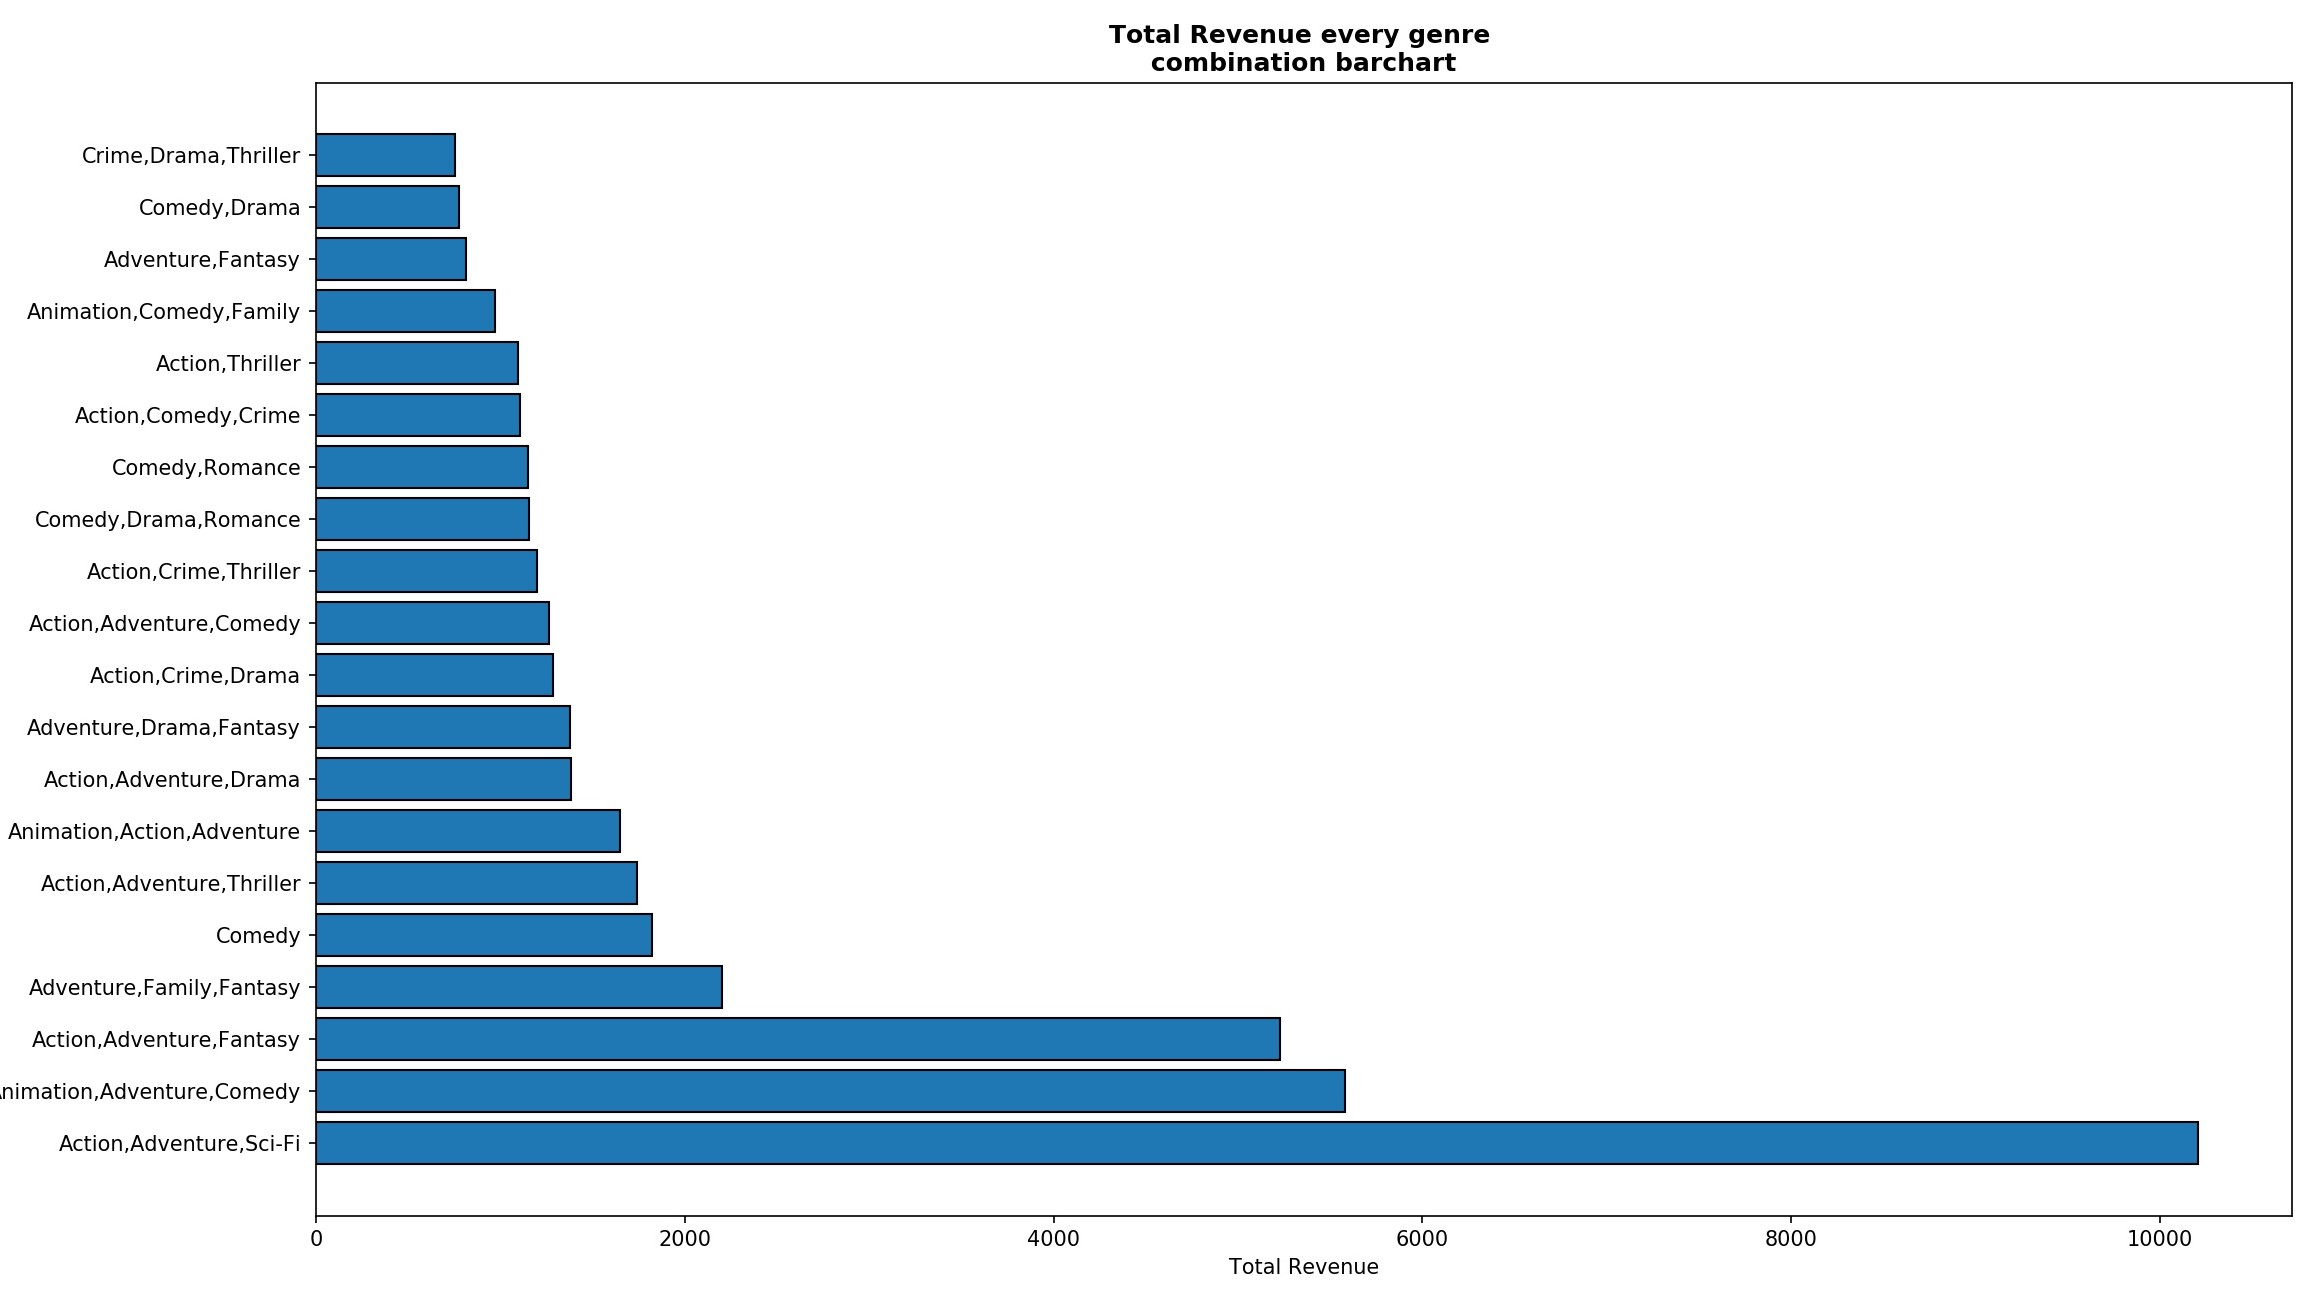
\includegraphics[scale=0.4]{./Lampiran/gambar/top20_genrecluster_totalRevenue_barchart}   
	\caption{20 Kombinasi genre dengan akumulasi \textit{revenue} tertinggi}
	\label{fig:top20_genrecluster_totalRevenue_barchart} 
\end{figure} 



\begin{figure}[H]
	\centering  
	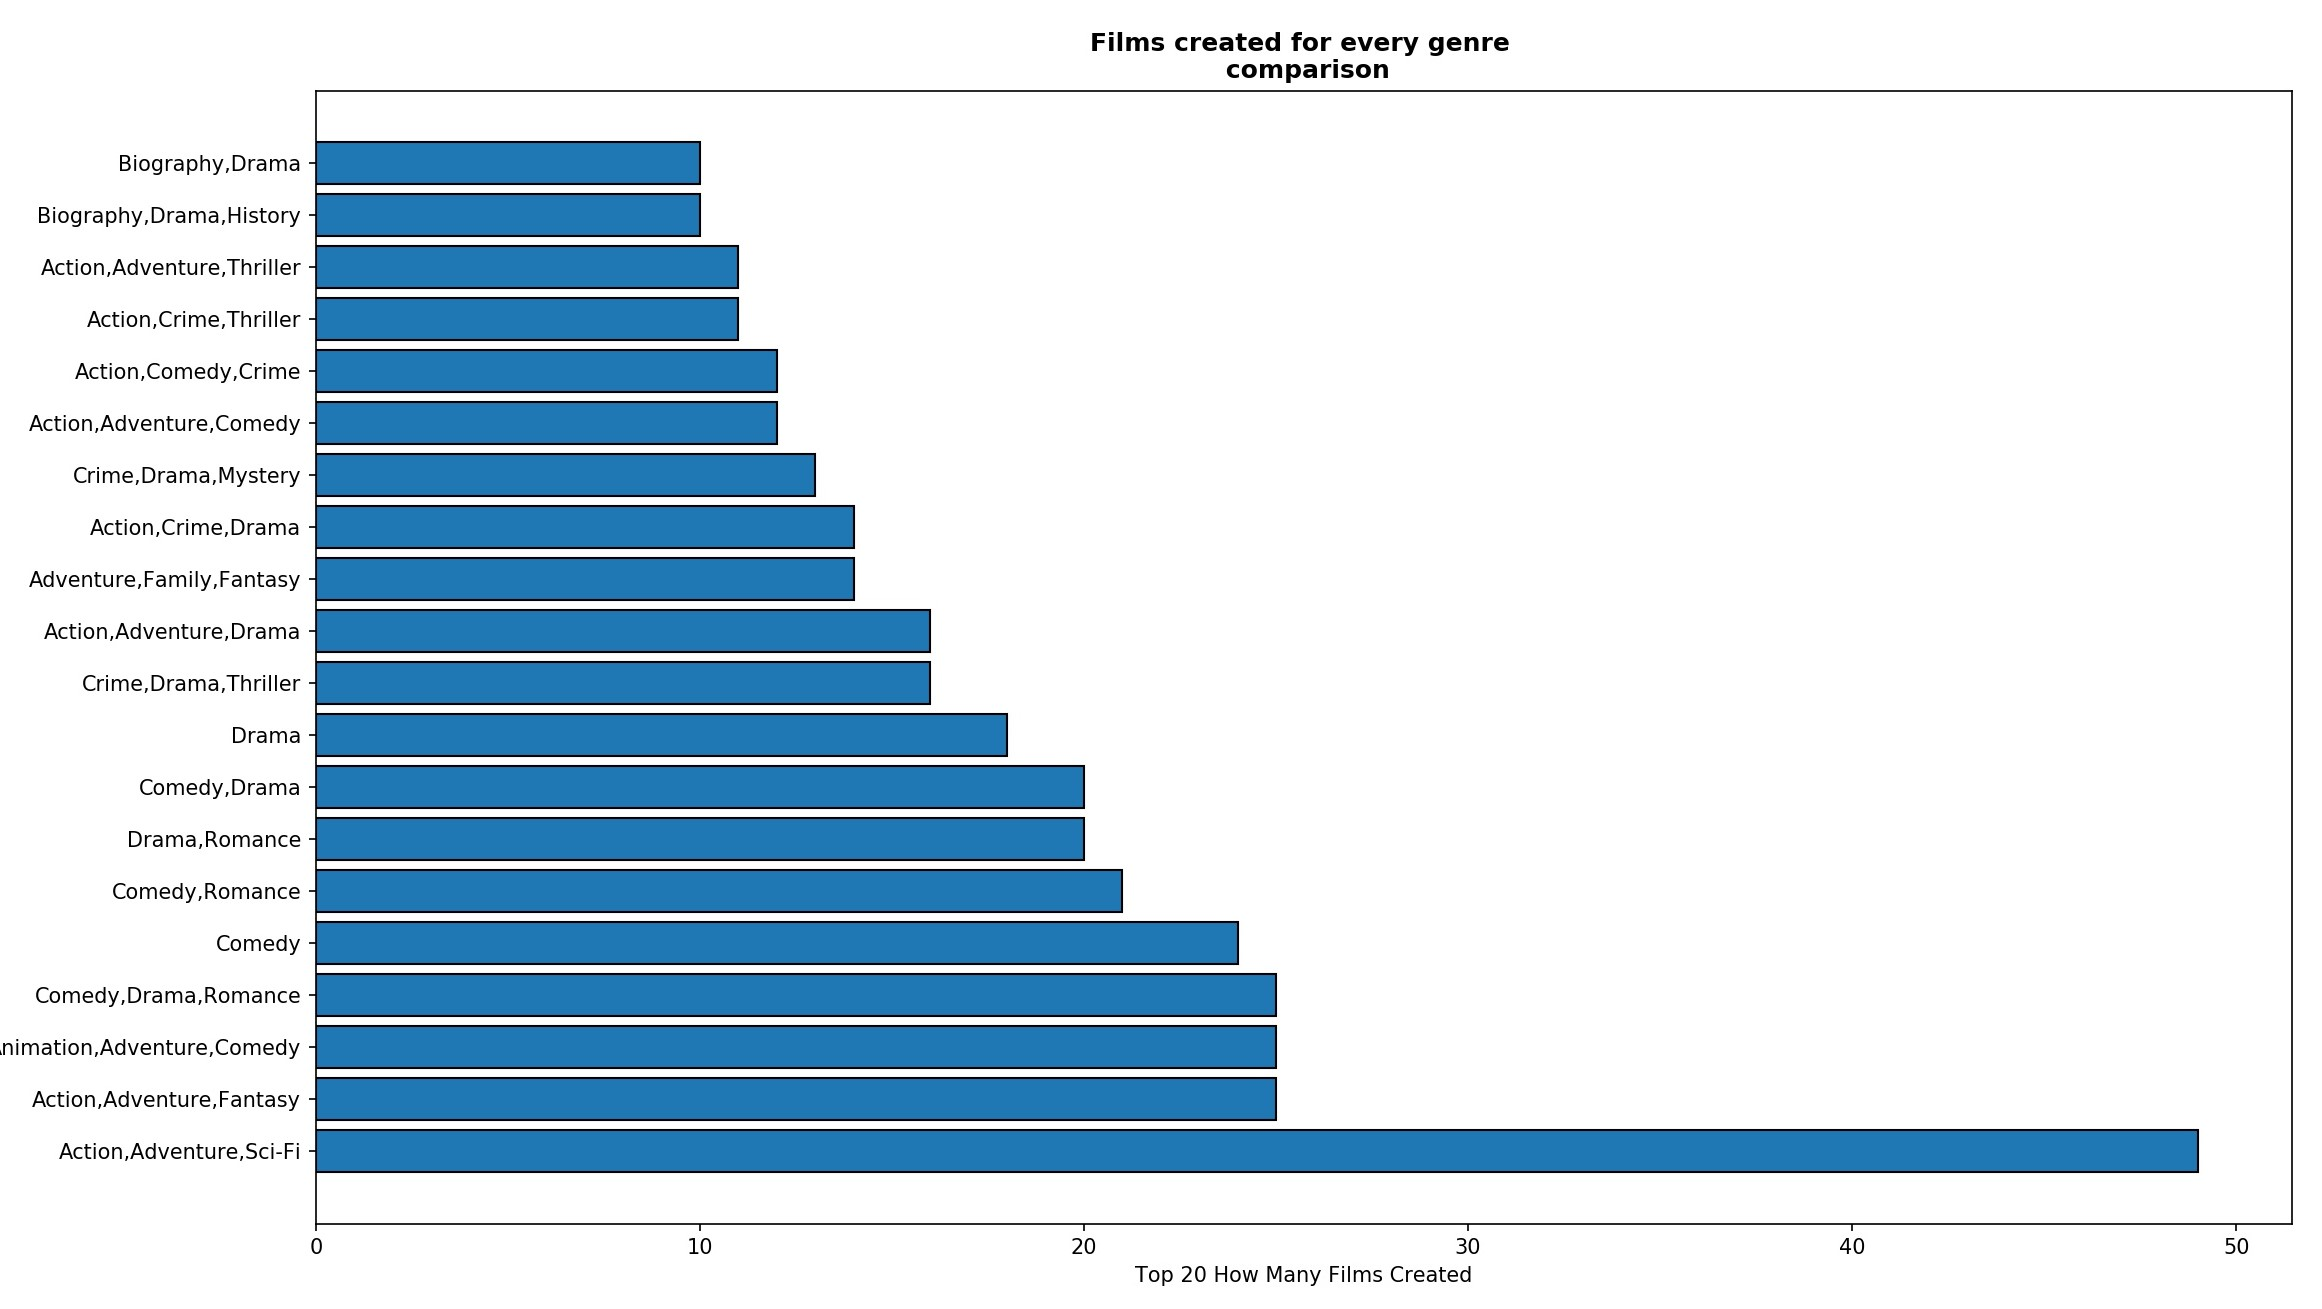
\includegraphics[scale=0.4]{./Lampiran/gambar/top20genrecluster_combinationtitle_barchart}   
	\caption{20 Kombinasi genre yang paling banyak dibuat}
	\label{fig:top20genrecluster_combinationtitle_barchart} 
\end{figure} 

\begin{figure}[H]
	\centering  
	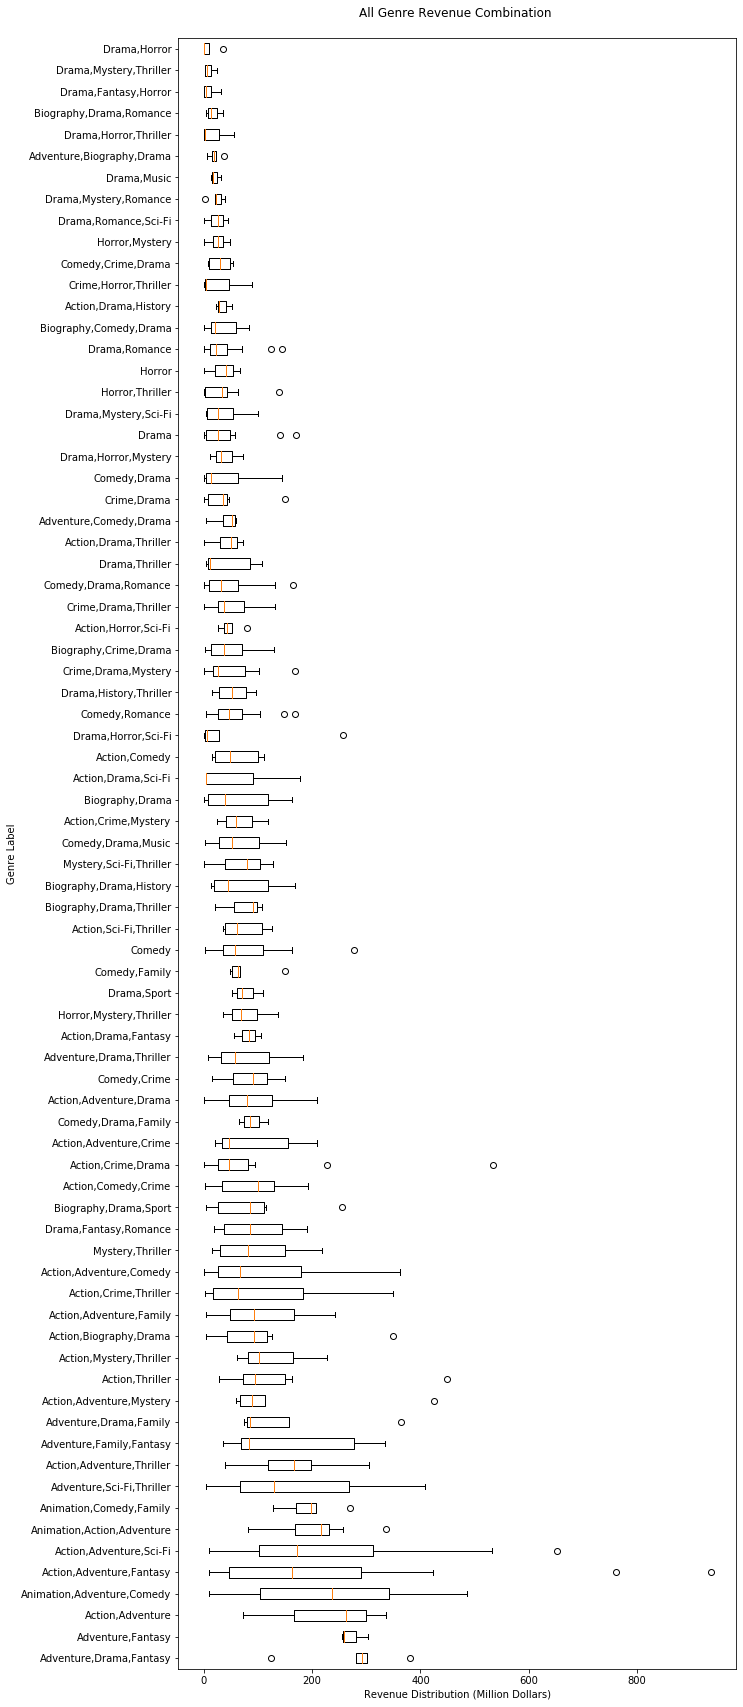
\includegraphics[scale=0.4]{./Lampiran/gambar/all_genre_multiboxplotbyrevenue}   
	\caption{Distribusi revenue semua kombinasi genre}
	\label{fig:all_genre_multiboxplotbyrevenue} 
\end{figure} 


\begin{figure}[H]
	\centering  
	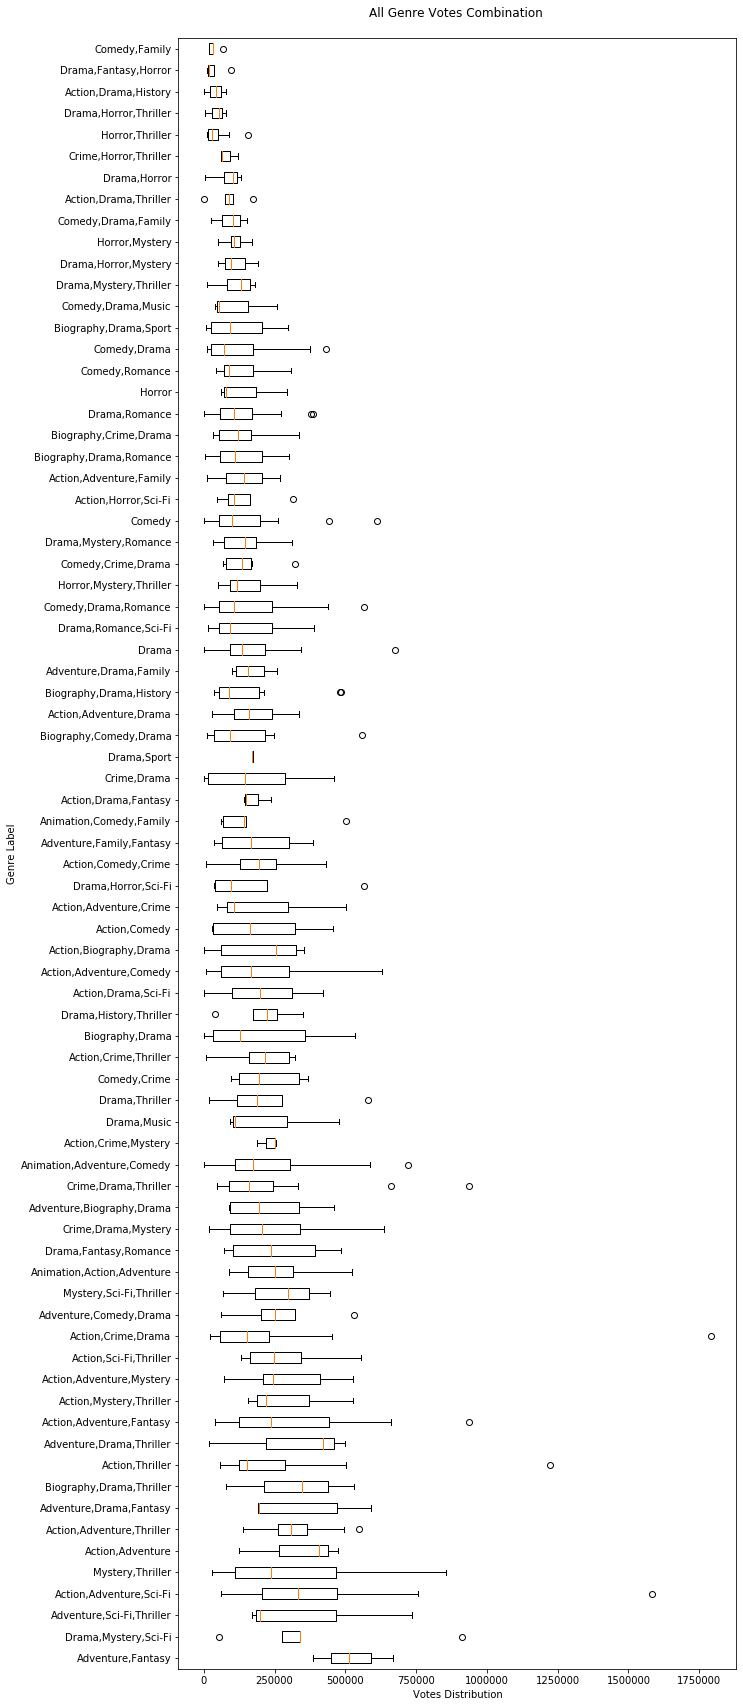
\includegraphics[scale=0.4]{./Lampiran/gambar/all_genre_multiboxplotbyvotes}   
	\caption{Distribusi votes semua kombinasi votes}
	\label{fig:all_genre_multiboxplotbyvotes} 
\end{figure} 


\begin{figure}[H]
	\centering  
	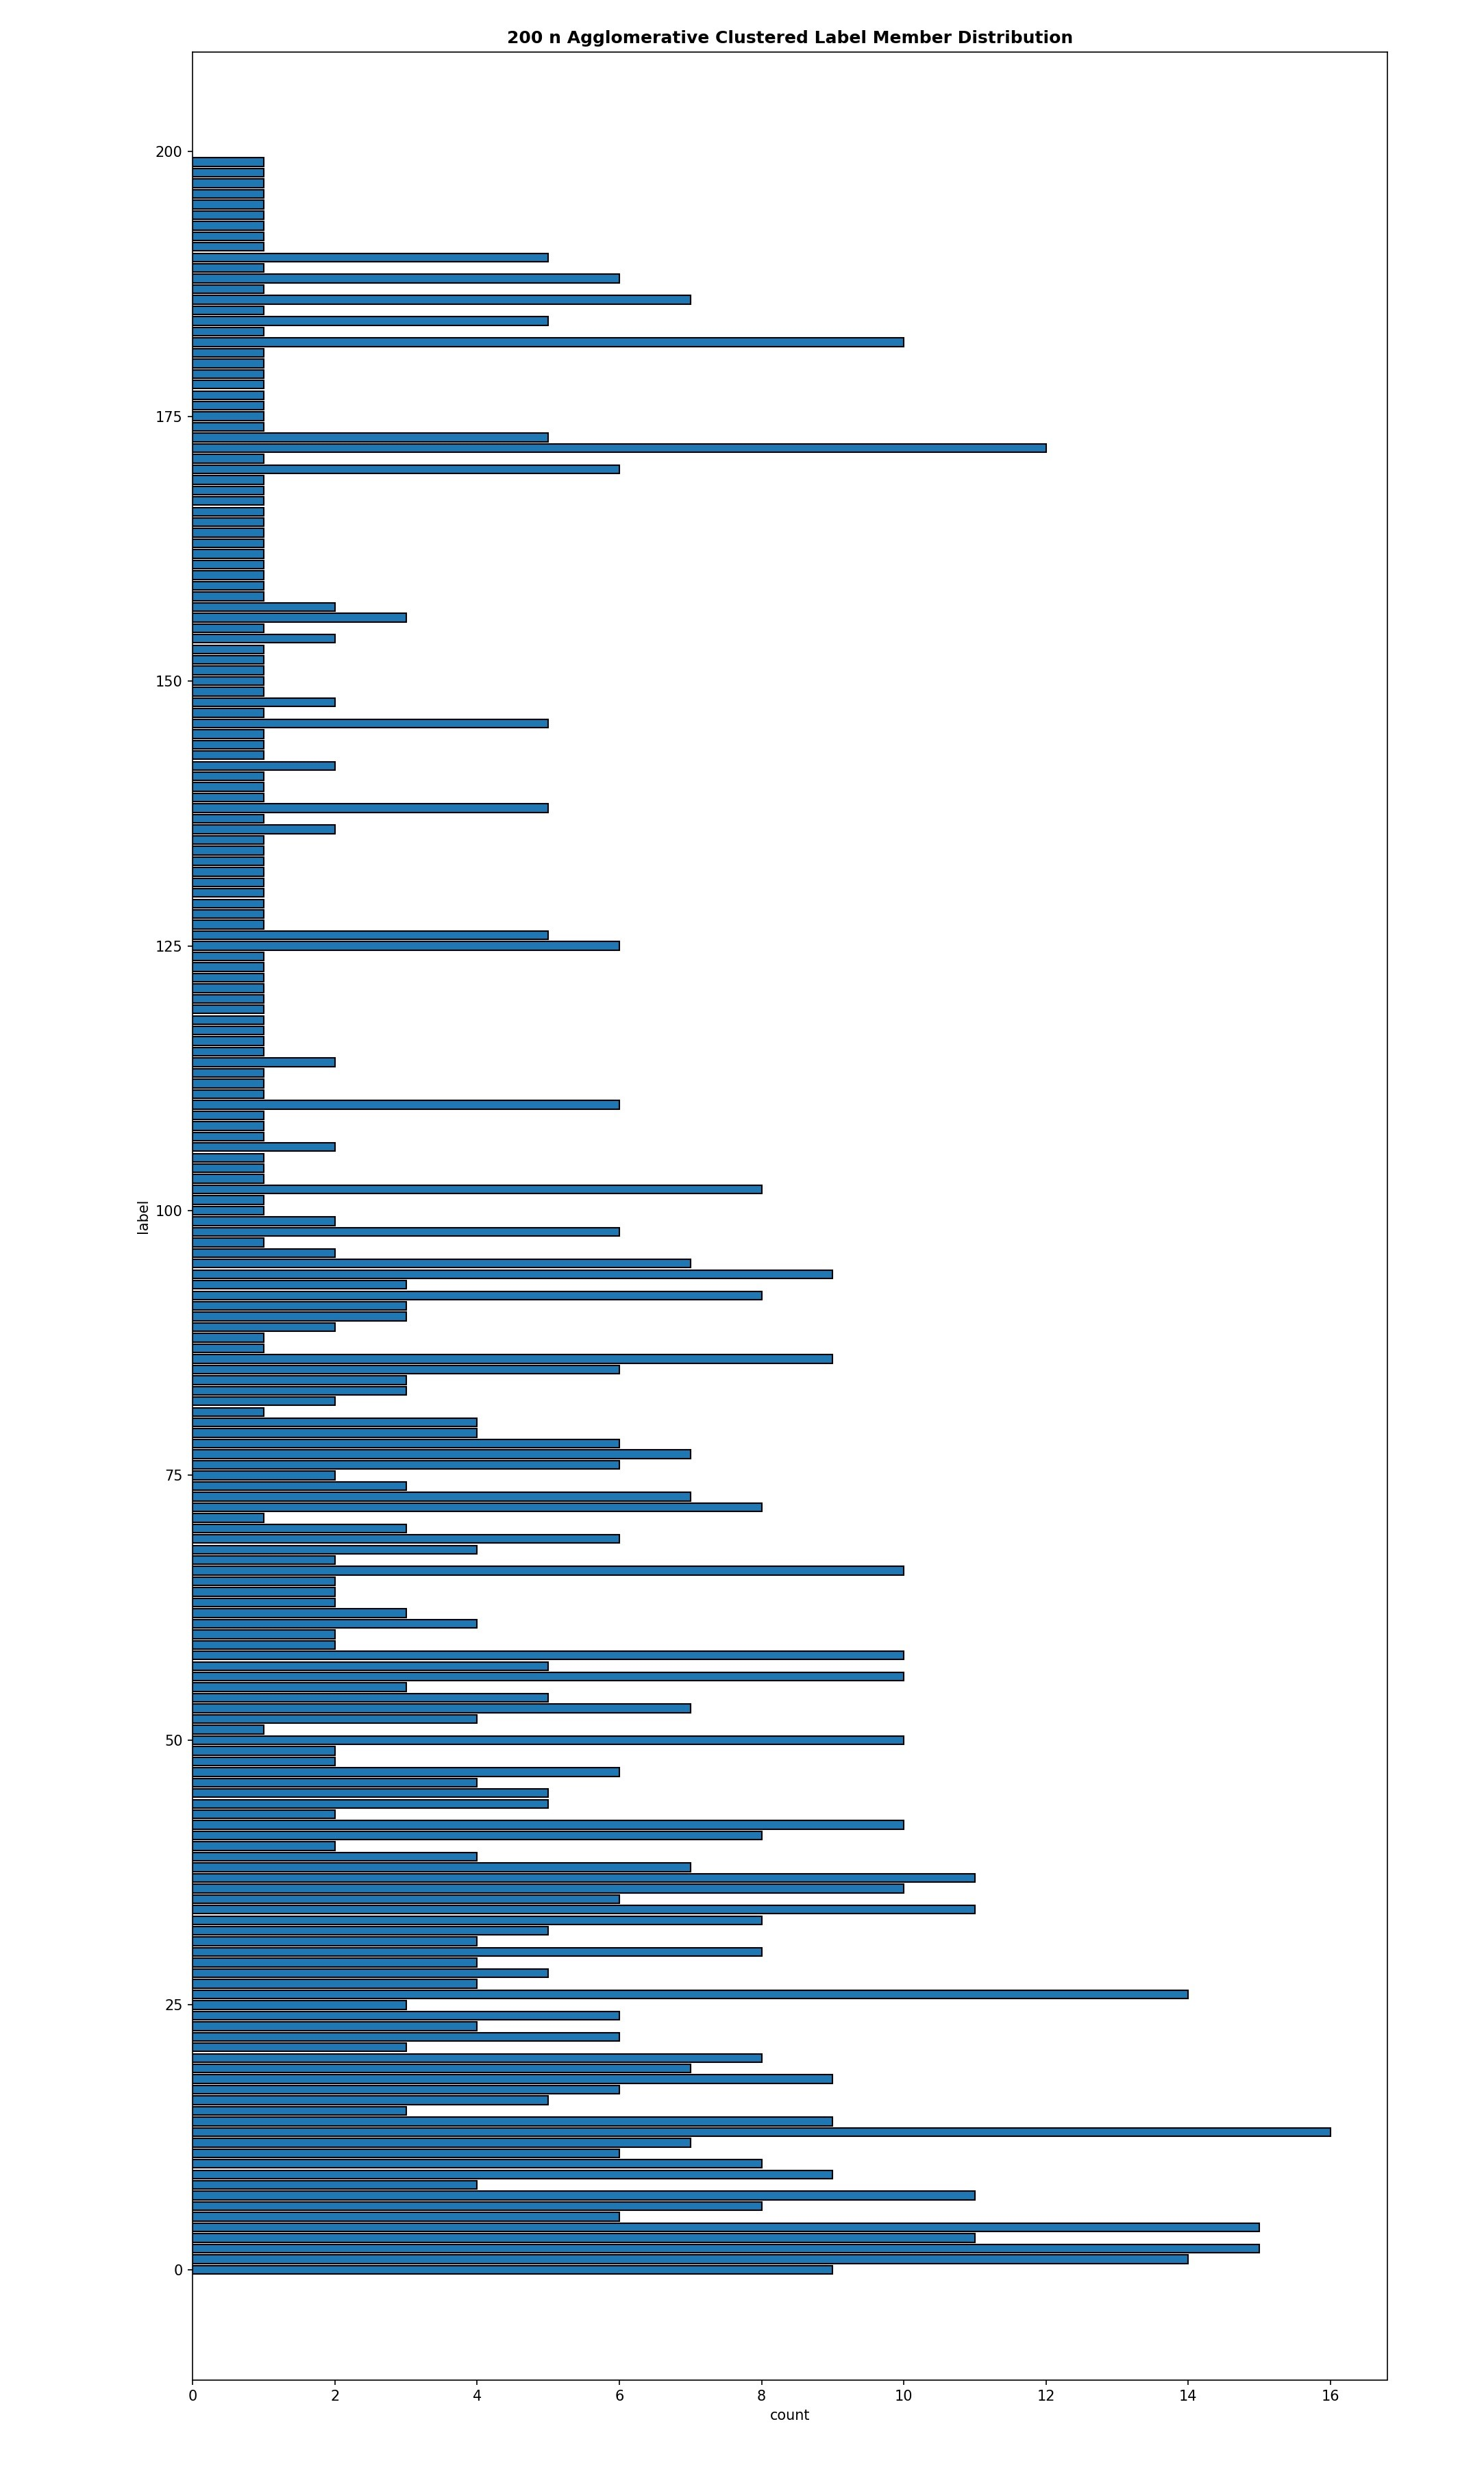
\includegraphics[scale=0.38]{./Lampiran/gambar/200_NAggloClusteredMemberLabelDistribution}   
	\caption{Distribusi Jumlah anggota hasil cluster aktor }
	\label{fig:200_NAggloClusteredMemberLabelDistribution} 
\end{figure} 

\begin{figure}[H]
	\centering  
	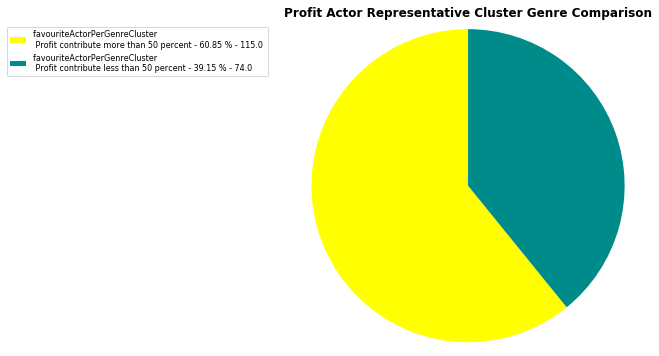
\includegraphics[scale=0.6]{./Lampiran/gambar/pieChartClusterGenre_FavActor_ProfitContributionComparison}   
	\caption{Jumlah perbandingan kelompok aktor yang genre favoritnya berkontribusi tertinggi pada \textit{profit} }
	\label{fig:pieChartClusterGenre_FavActor_ProfitContributionComparison} 
\end{figure} 


\begin{figure}[H]
	\centering  
	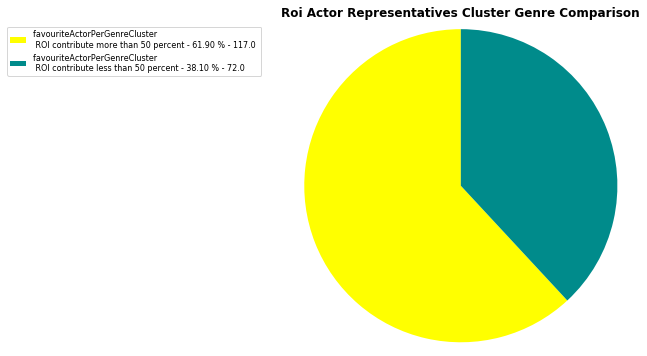
\includegraphics[scale=0.6]{./Lampiran/gambar/pieChartClusterGenre_FavActor_ROIContributionComparison}   
	\caption{Jumlah perbandingan kelompok aktor yang genre favoritnya berkontribusi tertinggi pada \textit{ROI} }
	\label{fig:pieChartClusterGenre_FavActor_ROIContributionComparison} 
\end{figure} 


